\ifdefined\iscombined
	\lecturetitle{Introduction}
\else
\documentclass{article}
\usepackage{xparse}
\usepackage{changepage}
\usepackage{listings}
\usepackage{amsthm}
\usepackage{comment}
\usepackage{amsmath}
\usepackage{braket}
\usepackage{amsfonts}
\usepackage{sectsty}
\usepackage{hyperref}
\usepackage{fancyhdr}
\usepackage[top=1in,bottom=1in,left=1in,right=1in]{geometry}
\usepackage{float}
\usepackage{graphicx}
\usepackage{mathtools}
\usepackage{tikz}
\usetikzlibrary{arrows}

\date{
	\vspace{-.75em}
	{\large \today}
}

\title{
	\vspace*{-1.5em}
	{\Huge Lecture 1} \\
	\vspace{-1em}
	\rule{\textwidth/4}{.01em} \\
	\vspace{-.25em}
	{\Large Introduction}
	\vspace{-.75em}
}

\author{
	{\large Matthew Farah}
}

\hypersetup{
	colorlinks=true,
	linkcolor=blue,
	filecolor=magenta,
	urlcolor=blue,
	citecolor=blue,
	anchorcolor=blue
}

\fancyhead{}
\fancyhead[L]{\today}
\fancyhead[R]{Lecture 1 - Introduction}

\setlength{\parindent}{0cm}

\newcounter{example}
\renewcommand{\theexample}{\arabic{example}}

\newenvironment{example}[1][]{
	\refstepcounter{example}
	\begin{adjustwidth}{1.5em}{}
	\noindent\textbf{\ifx&#1&Example \theexample:\else Example \theexample \ (#1):\fi}
	\ignorespaces
}{
	\vspace{.5em}
	\end{adjustwidth}
}

\newenvironment{solution}{
	\vspace{.5em}
	\par
	\begin{adjustwidth}{1.5em}{}
	\textbf{{Solution:}}
	\par
	\vspace{.5em}
}{
	\vspace{1em}
	\end{adjustwidth}
}

\newcounter{subexample}
\renewcommand{\thesubexample}{\alph{subexample}}

\newenvironment{subexample}{
	\setcounter{step}{0}
	\refstepcounter{subexample}
	\vspace{1em}\par\noindent
	\begin{adjustwidth}{1.5em}{}
	\noindent\textbf{(\thesubexample)}
	\ignorespaces
}{
	\par
	\vspace{1em}
	\end{adjustwidth}
}

\renewenvironment{proof}{
	\vspace{.5em}\par\noindent
	\begin{adjustwidth}{1.5em}{}
	\emph{Proof:}\par\vspace{1em}
	\setlength{\parindent}{0cm}
}{
	\end{adjustwidth}
}

\newtheorem{theorem}{Theorem}

\renewenvironment{theorem}[1][]{
	\refstepcounter{theorem}
	\vspace{1em}\par\noindent
	\begin{adjustwidth}{1.5em}{}
	\noindent\textbf{\ifx&#1&Theorem \thetheorem:\else Theorem \thetheorem \ (#1):\fi}
	\ignorespaces
}{
	\vspace{.5em}
	\end{adjustwidth}
}

\newtheorem{lemma}{Lemma}

\renewenvironment{lemma}[1][]{
	\refstepcounter{lemma}
	\vspace{1em}\par\noindent
	\begin{adjustwidth}{1.5em}{}
	\noindent\textbf{\ifx&#1&Lemma \thelemma:\else Lemma \thelemma \ (#1):\fi}
	\ignorespaces
}{
	\vspace{.5em}
	\end{adjustwidth}
}

\makeatother
\makeatletter

\newcounter{step}
\renewcommand{\thestep}{\Roman{step}}

\newenvironment{step}{
	\refstepcounter{step}
	\vspace{1em}\par\noindent
	\ignorespaces\noindent\textbf{(\thestep)}
	\ignorespaces
}{
	\par
}

\sectionfont{\fontsize{12}{12}\bfseries}
\subsectionfont{\fontsize{10}{12}\normalfont}
\subsubsectionfont{\fontsize{10}{12}\normalfont}

\begin{document}

\maketitle
\pagestyle{fancy}

\fi

\begin{itemize}
	\item A control system is used to produce an output for a given input.
	\item Control systems can be represented by the following black-box diagram:
\end{itemize}

\vspace{1em}

\begin{figure}[H]
	\centering
	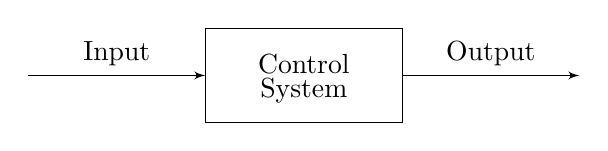
\begin{tikzpicture}[>=latex']
		\draw[->] (-3.5,0) -- (-1.25,0);
		\node[above] at (-2.375,0) {Input};
		\draw (-1.25,-0.6) rectangle (1.25,0.6);
		\node at (0,0.15) {Control};
		\node at (0,-0.2) {System};
		\draw[->] (1.25,0) -- (3.5,0);
		\node[above] at (2.375,0) {Output};
	\end{tikzpicture}
\end{figure}

\vspace{1em}

\begin{itemize}
	\item An open loop system is a control system without feedback.
	\item A closed loop system is a control system with feedback.
	\item The transient response of a control system describes a system's behaviour before reaching steady state in response to some input.
	\item The steady state response of a control system describes the long-run behaviour of a control system in response to some input.
	\item The steady state error is defined to be the discrepancy between the control system's desired steady state and its actual steady state.
	\begin{itemize}
		\item Good control systems minimize their steady state error as much as possible.
	\end{itemize}
	\item The natural response of a control system is defined as the evolution of the control system's output due to its initial conditions.
	\item The forced response of a control system is defined as the evolution of the control system's output due to its input.
	\item The total response of a system is defined to be the sum of the system's natural and forced response.
	\begin{itemize}
		\item Total response = natural response + forced response.
	\end{itemize}
	\item A system is said to be stable if its natural response tends to zero.
	\begin{itemize}
		\item Good control systems, at worst, have a natural response which oscillates around zero at a fixed amplitude.
	\end{itemize}
	\item The goals of good control system design are five-fold:
	\begin{enumerate}
		\item Ensure the system is stable.
		\item Produce the desired transient response.
		\item Decrease/eliminate the steady state error.
		\item Make the system robust enough to withstand disturbances.
		\item Optimize performance.
	\end{enumerate}
\end{itemize}

\ifdefined\iscombined
	\newpage
\else
	\end{document}
\fi
